% !TeX spellcheck = de_DE
\documentclass[aspectratio=169]{beamer}

\usetheme[progressbar=frametitle]{metropolis}
\usepackage{appendixnumberbeamer}

\usepackage{booktabs}

\usepackage{pgfplots}
\usepgfplotslibrary{dateplot}

\usepackage{soul}
\usepackage{xspace}

\titlegraphic{\hfill
\includegraphics[height=3.5cm]{img/logo}}


\title{OpenShift / Keycloak SSO / Kong}
\subtitle{Nachmittag Session}

\date{17. August 2018}

\author{Tobias Derksen \& Gerald Schmidt}
\institute{codecentric AG / Berlin}

\begin{document}

% Title Frame
\maketitle

% Agenda
\begin{frame}{Agenda}
	\setbeamertemplate{section in toc}[sections numbered]
	\tableofcontents[hideallsubsections]
\end{frame}


% !TeX spellcheck = de_DE
\section{Authentication Basics}


\begin{frame}{Authentication vs. Authorization}
	\metroset{block=fill}
	\begin{block}{Authentication}
		Authentication is the process of ascertaining that somebody really is who he claims to be. \\
		\textit{$\Longrightarrow$ login + password (who you are)}
	\end{block}

	~\\

	\begin{block}{Authorization}
		Authorization refers to rules that determine who is allowed to do what. \\
		\textit{$\Longrightarrow$ permissions (what you are allowed to do)}
	\end{block}	
\end{frame}


\begin{frame}{Methods \& Protocols}
	\begin{itemize}
		\item Single-Sign-On (SSO)
		\item OAuth \& OpenID Connect (OIDC)
		\item JSON Web Token (JWT)
		\item Access Token \& Refresh Token
	\end{itemize}
\end{frame}


% !TeX spellcheck = de_DE
\section{Keycloak  SSO}


\begin{frame}{Über Keycloak}
	\begin{itemize}
		\item Open Source
		\item Single-Sign-On / Identity Management
		\item Java
		\item JBoss / Wildfly
	\end{itemize}
\end{frame}

\begin{frame}{Terminologie}
	\begin{itemize}
		\item Realms
		\item Clients
		\item User
		\item User Federation / Identity Provider
		\item Authentication Flow
	\end{itemize}
\end{frame}

\begin{frame}{Authorization}
	\begin{itemize}
		\item Roles / Client Roles
		\item Groups
		\item Scopes / Client Scopes
	\end{itemize}
\end{frame}


\begin{frame}[standout]
Hands-On Keycloak
\end{frame}
% !TeX spellcheck = de_DE
\section{Kong API Gateway}


\begin{frame}{Über Kong}
\begin{columns}
	\column{0.5\textwidth}
		\begin{itemize}
		\item API Verwaltung
		\item Analysiere \& Modifiziere Requests
		\item Plugins für erweiterte Funktionen
		\item Open Source
	\end{itemize}

	\column{0.5\textwidth}
	\begin{itemize}
		\item Nginx
		\item Cassandra / PostgreSQL
		\item Administration via REST
	\end{itemize}
\end{columns}
\end{frame}

\begin{frame}{Terminologie}
	\begin{figure}
		\centering
		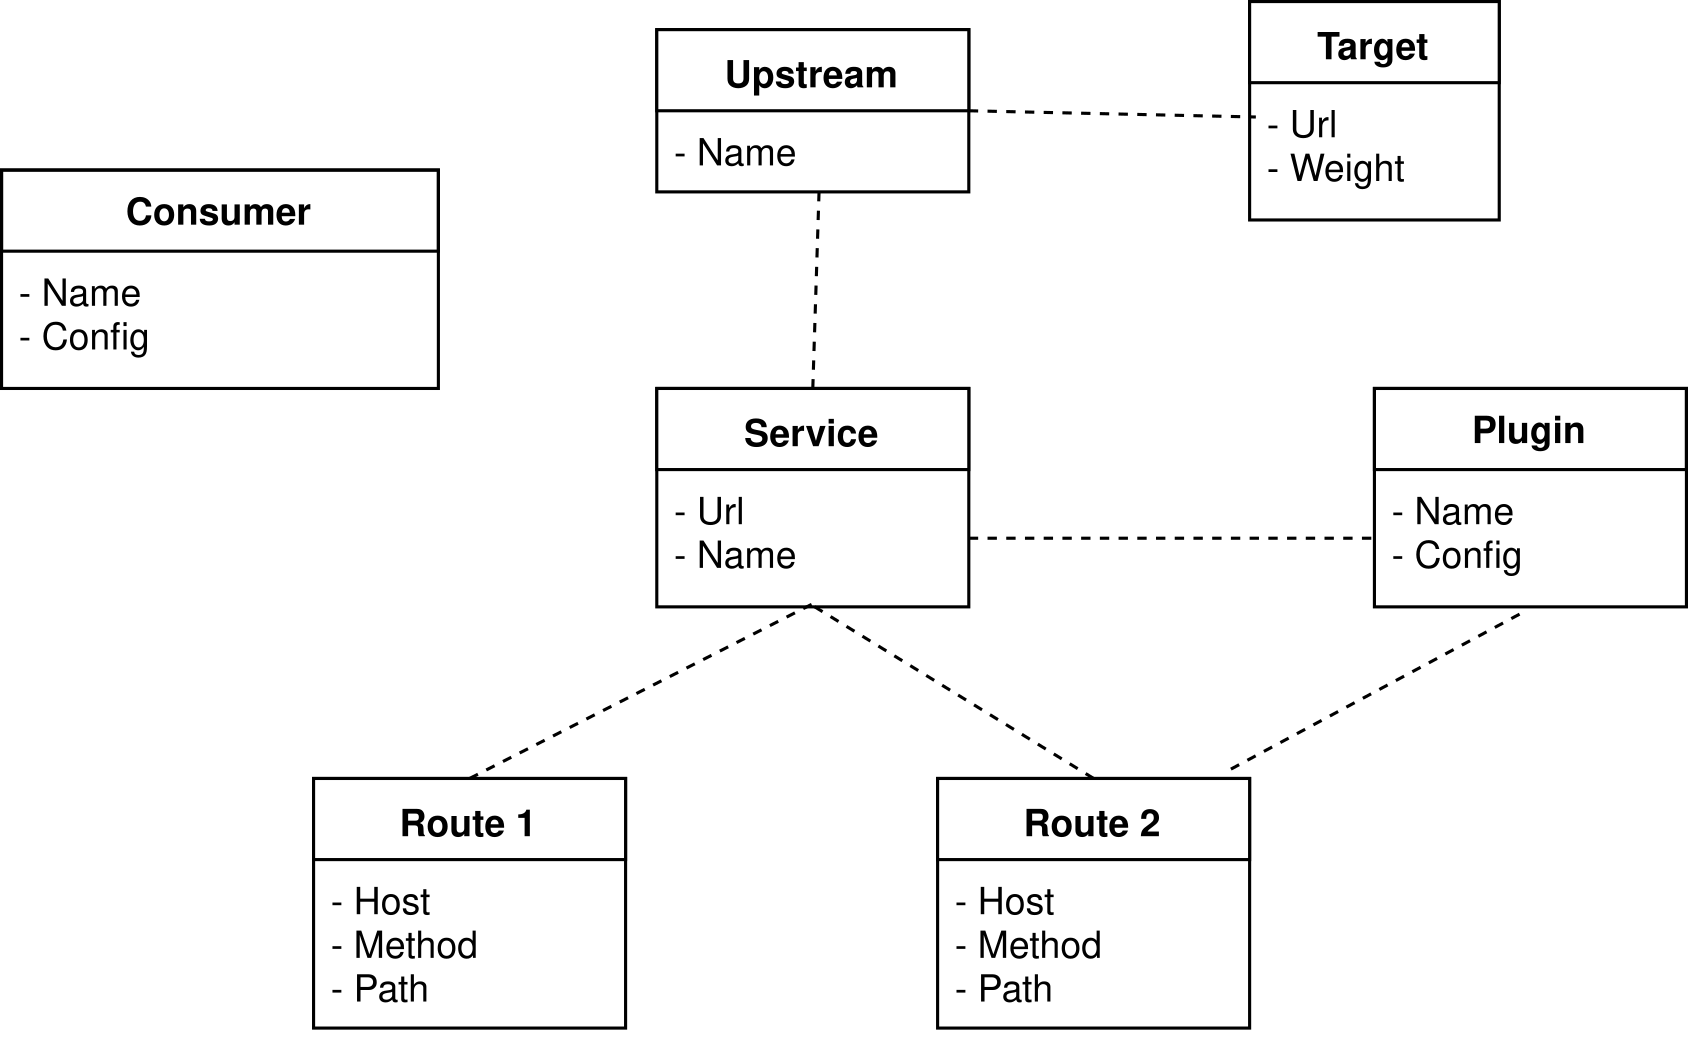
\includegraphics[width=0.75\linewidth]{img/kong_overview}
	\end{figure}
\end{frame}

\begin{frame}{Kong Load Balancing}
	\begin{itemize}
		\item DNS based (SRV, A, CNAME)
		\item Round Robin / Ring Buffer
		\item Weighted
	\end{itemize}
\end{frame}

\begin{frame}[standout]
	Hands-On Kong
\end{frame}





\begin{frame}{Microservice Architektur}
	\begin{figure}
		\centering
		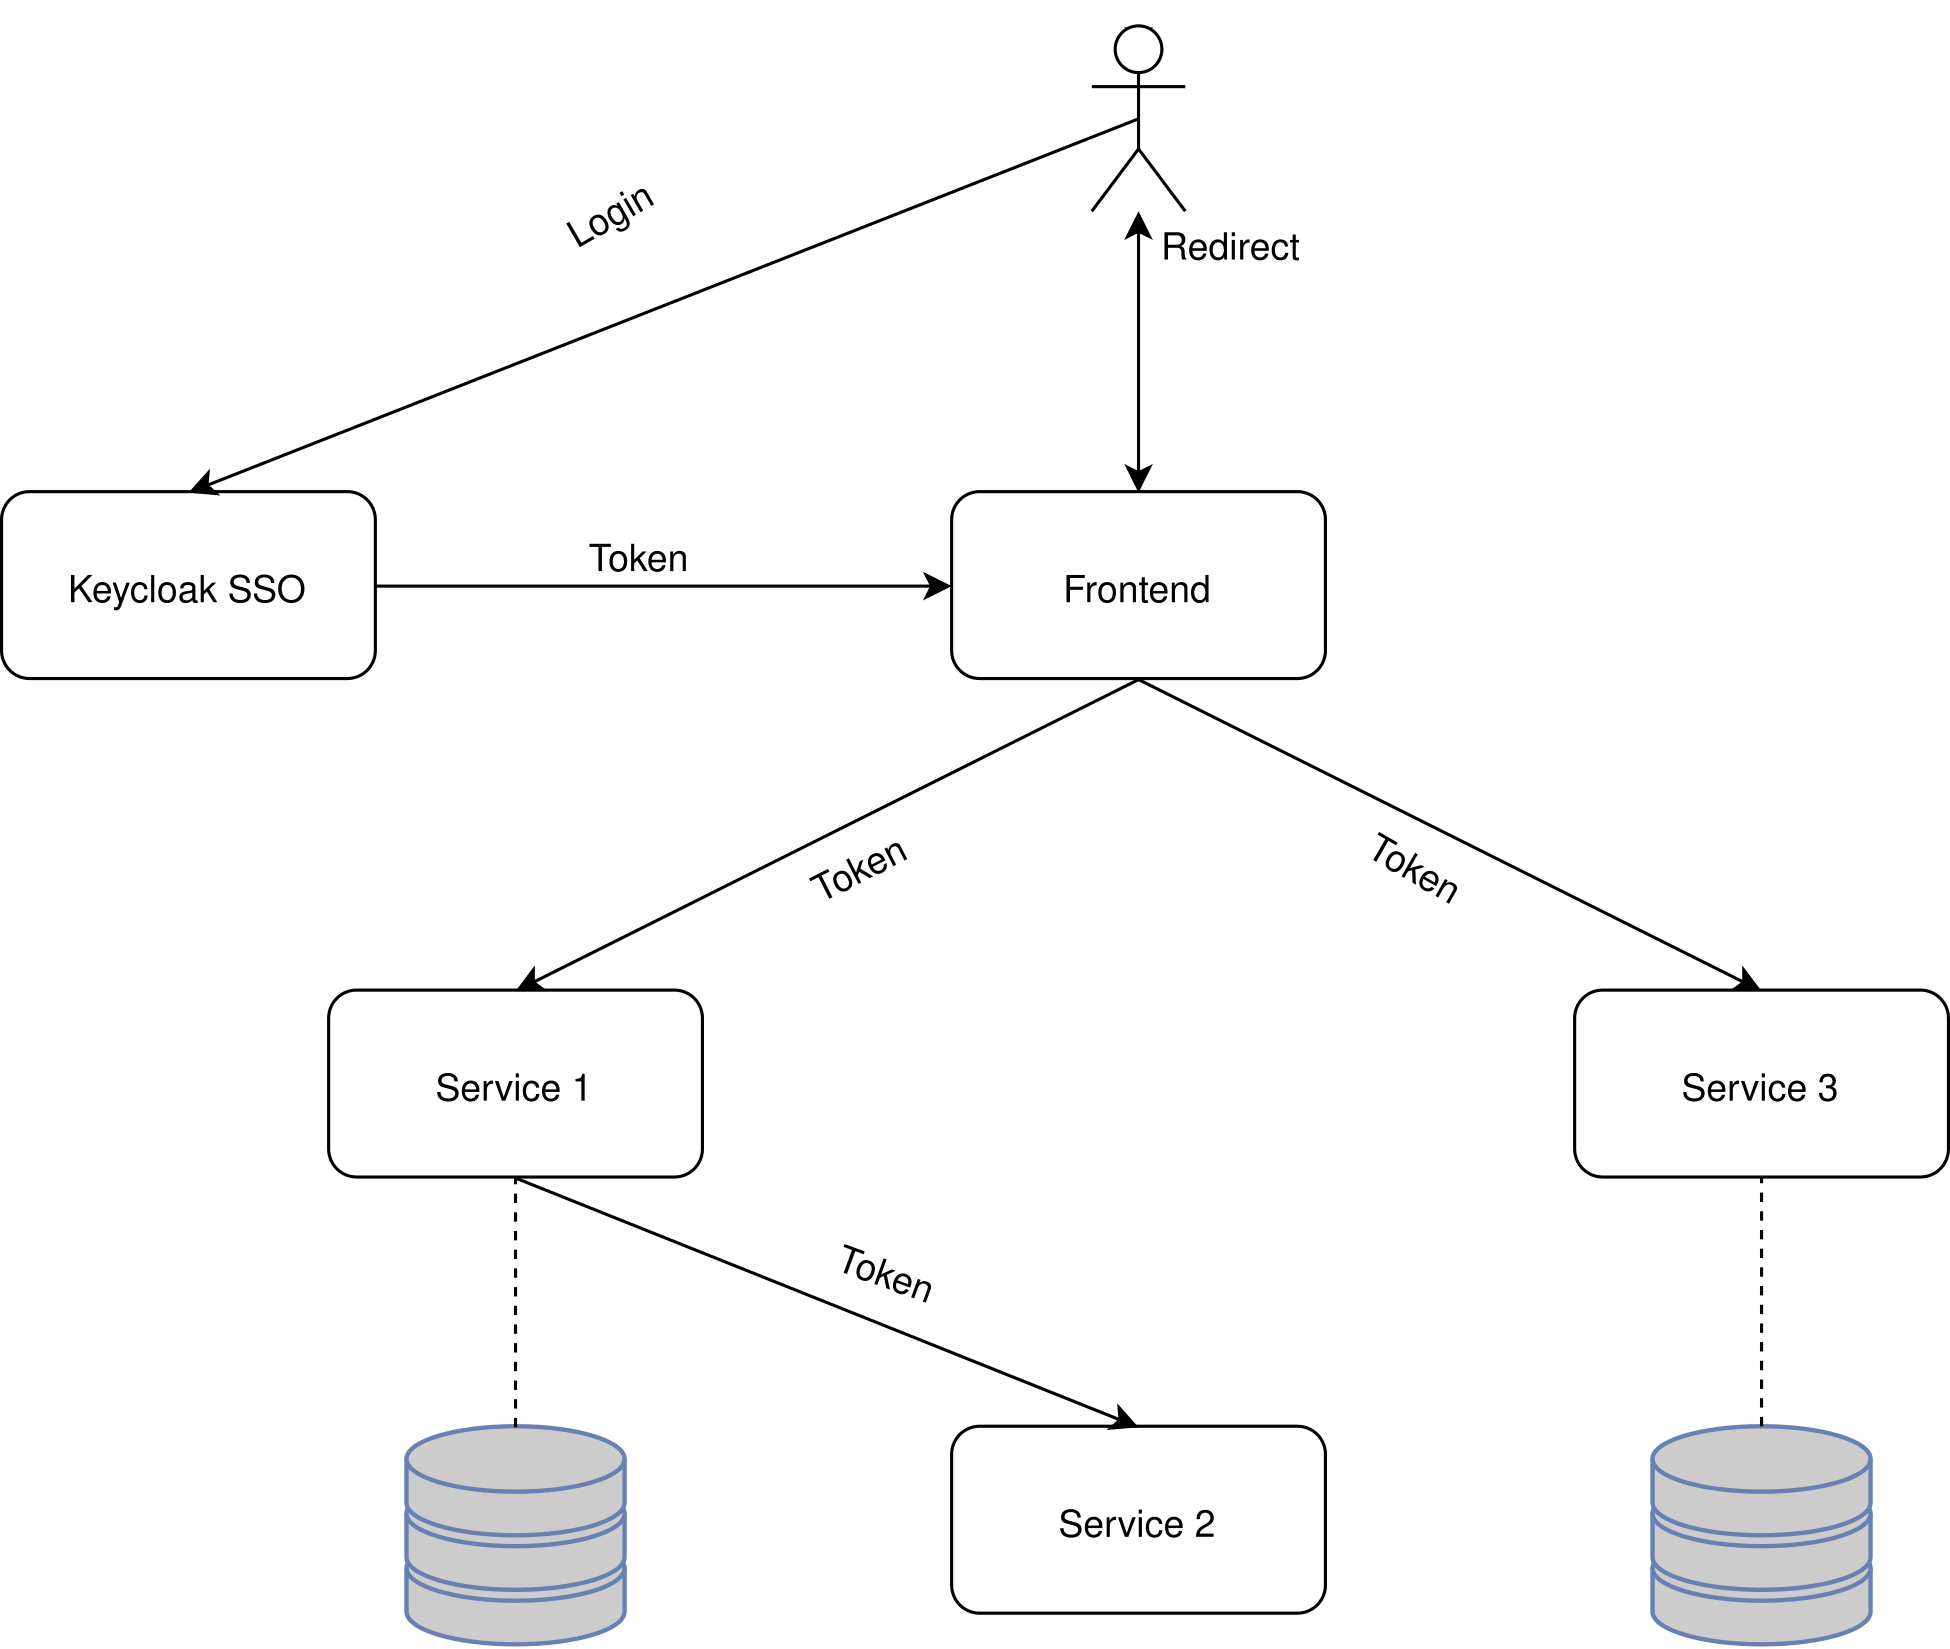
\includegraphics[height=0.85\textheight]{img/setup_basic}
	\end{figure}
\end{frame}


\begin{frame}{Microservice Architektur (mit Kong)}
	\begin{figure}
		\centering
		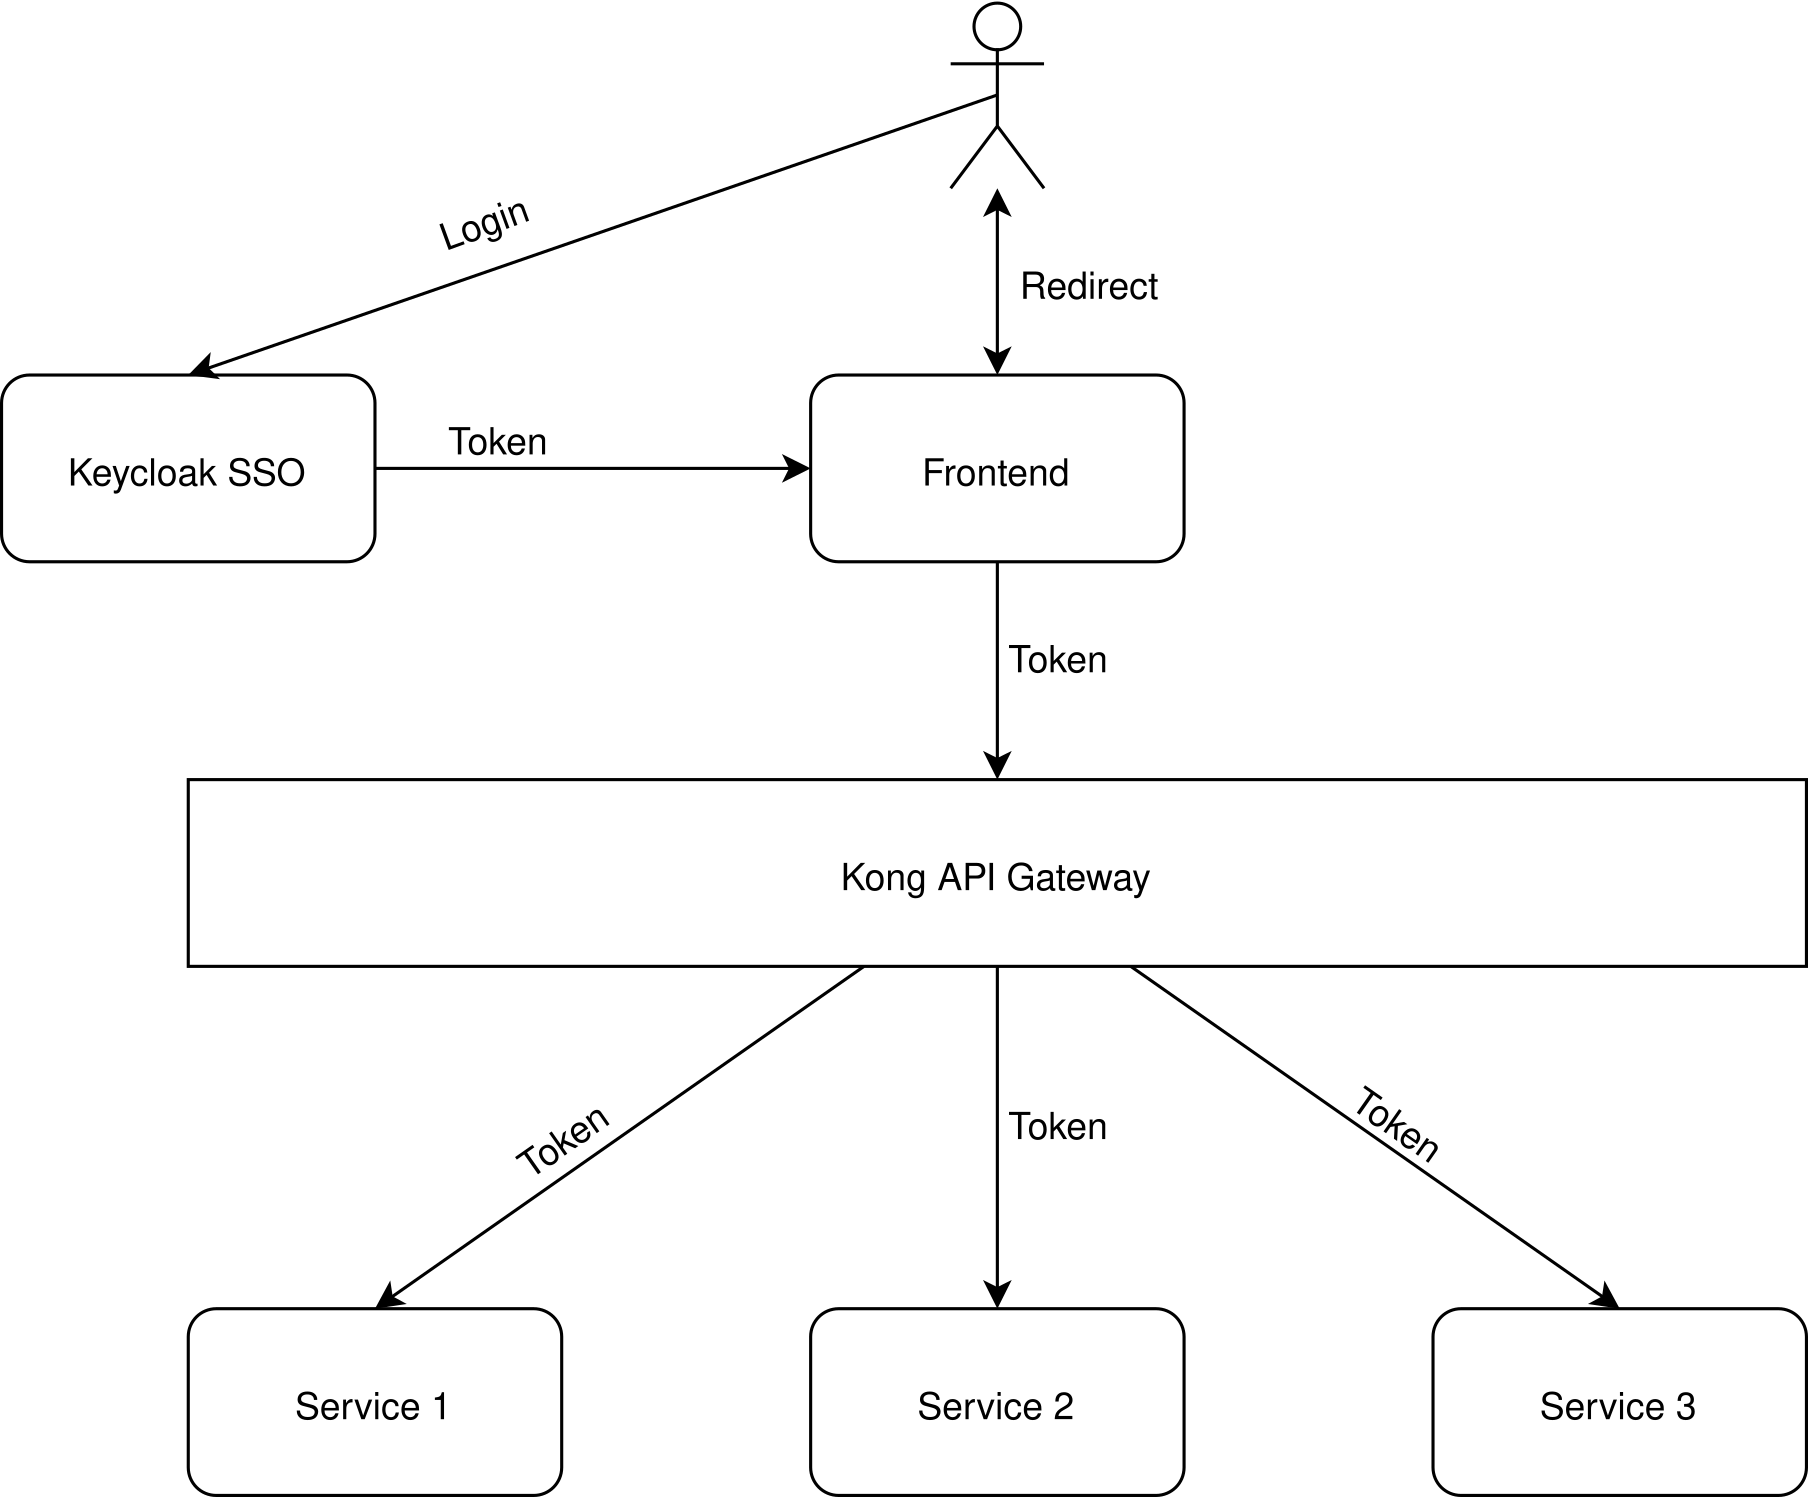
\includegraphics[height=0.85\textheight]{img/setup_kong}
	\end{figure}
\end{frame}


\begin{frame}[standout]
Integrated Prototype
\end{frame}


% !TeX spellcheck = de_DE
\section{Advanced Topics}


\begin{frame}{High Availability}
	\begin{itemize}
		\item Databases
		\item Keycloak
		\item Kong
	\end{itemize}
\end{frame}


\begin{frame}{Advanced Topics}
	\begin{itemize}
		\item Secure Kong Admin API
		\item Statelessness (PHP Session!!!)
		\item API Versioning
		\item Request Logging
	\end{itemize}
\end{frame}



\end{document}